% Centro de Estadística y Matemática Aplicada
% Universidad Simón Bolívar
% Plantilla LaTeX para manuscritos (tesis y pasantías)
% pregrado y postgrado
%
% Andrés M. Sajo-Castelli
% Carlos Contreras
%
% 15 Abril 2015 -- primera versión pública
% ...
% 11 Mayo 2018 --- Se agrega bibliografía en castellano via babelbib
%
\documentclass[pregrado]{tesis-usb}

% paquetes
\usepackage[utf8]{inputenc}
\usepackage[utf8]{inputenc}
\usepackage{ragged2e}
\usepackage{indentfirst}
\usepackage{longtable}
\usepackage{tabu}
\usepackage{float}
\usepackage{hhline}
\usepackage{makecell}
\usepackage{multirow}
\usepackage{array}
\usepackage{verbatim}
\usepackage{acronym}
\usepackage{amsmath}
\usepackage{amsfonts}
\usepackage{amssymb}
\usepackage{float}
\usepackage{pdfpages}
\usepackage{xcolor}
\definecolor{red}{HTML}{FF4C4C}
% \usepackage{hyperref}

% estilo de las referencias
\usepackage[fixlanguage]{babelbib-and}\selectbiblanguage{spanish}
\usepackage{url}
\bibliographystyle{IEEEtran}

\usepackage{graphicx}
% \graphicspath{ {../imgs/} }

\autor{Valentina Hernández}
\autori{V. Hernández}
\usbid{10-10353}
\titulo{Desarrollo de la versión 2 de la aplicación web CPI}
\fecha{Septiembre~de~2018}
\agno{2018}
\fechadefensa{30~de~noviembre~de~2018}
\tutor{Tutor Académico: Prof. Soraya Carrasquel}
\usarcotutor
\cotutor{Tutor Industrial: Ing. José Cerqueiro}
\trabajo{Informe de Pasantía}
\coord{Ingeniería de la Computación}
\grado{Ingeniero de la Computación}
\carrera{Ingenieria de la Computación}
\programa{Nombre del Programa}
\juradouno{Nombre y Apellido}
\juradodos{Nombre y Apellido}
\juradotres{Nombre y Apellido}

% Cambia comillas simple por comilla cerrada en ambiente verbatim
\makeatletter
\let \@sverbatim \@verbatim
\def \@verbatim {\@sverbatim \verbatimplus}
{\catcode`'=13 \gdef \verbatimplus{\catcode`'=13 \chardef '=13 }}
\makeatother

\begin{document}

\frontmatter
\maketitle
\begin{resumen}
     Es una exposici\'on clara del tema tratado en el trabajo, de los objetivos, de la metodolog\'ia utilizada, de los resultados relevantes obtenidos y de las conclusiones. Mismo tipo de fuente seleccionado con tamaño 12 e interlineado sencillo en el p\'arrafo. El resumen no debe exceder de trescientas (300) palabras escritas. \\
     Palabras cl\'aves: palabras, cl\'aves, separadas por coma, cinco m\'aximo.
\end{resumen}
\tableofcontents
\listoffigures

\mainmatter
\chapter*{Introducción}
\par Introducción aquí.
\chapter{Entorno empresarial} \label{empresa}
En este capítulo se presenta una descripción del entorno en el cual se desarrolló el proyecto de pasantía en la empresa iKêls Consulting. Comprende una breve reseña histórica, su misión y visión, la estructura organizacional y el área a la cual el pasante estuvo asignado.

\section{Antecedentes de la empresa}
IKêls Consulting \cite{ikels} se creó el año 2008 como una empresa dedicada al desarrollo de soluciones en el área de Sistemas de Información. Los fundadores contaban con una amplia trayectoria en los procesos y tecnología para la elaboración de documentación técnica avanzada (por ejemplo normas ISO para construcción de plantas petroquímicas).

Para aprovechar la experiencia previa los productos y servicios se concentran en el área de aplicaciones web (por ejemplo, sistemas de manejo de contenido o CMS \cite{cmsBarker}) para el sector corporativo atendiendo a un selecto grupo de clientes con presencia local e internacional.

Actualmente, las actividades principales se concentran en:

\begin{itemize}
  \item Construcción de portales web en múltiples idiomas y que pueden ser administrados por sus propios dueños. Esto incluye la programación de módulos especiales para integrar información desde y hacia sistemas externos, desplegar datos de manera amigable o generar notificaciones automáticas dependientes de actividades de los visitantes u otros eventos.
  \item Apoyo en la gestión de contenido de portales web.
  \item Consultoría y gestión para optimizar las variables asociadas al rendimiento y desempeño de las páginas web. Teniendo especial interés en el monitoreo de presencia en buscadores, evaluación del perfil de los visitantes y garantizar un nivel adecuado de usabilidad en diferentes dispositivos, etc.
  \item Desarrollo de productos personalizados que complementen las ventajas y facilidades de los dispositivos móviles en sincronización con mecanismos de soporte en servidores web.
  \item Desarrollo de soluciones especializadas para ofrecer bajo el modelo SaaS o \textit{Software as a Service} (Software como servicio) \cite{saas}.
\end{itemize}

\section{Misión}
Proveer productos y servicios en el área de sistemas de información que permitan una comunicación efectiva de nuestros clientes con su público y también sirva como plataforma de trabajo donde se aprovechen las innovaciones y ventajas de las tecnologías más modernas.

\section{Visión}
Deseamos ser un proveedor confiable, que ofrece un alto valor agregado en cada producto o servicio que prestamos a nuestros clientes.

\section{Ubicación del pasante}
El proyecto de pasantía pertenece al grupo de Desarrollo de Aplicaciones y cuenta con la dirección del Presidente de la Empresa y con el apoyo de los ingenieros líderes del grupo. A continuación se muestra el organigrama de la empresa.


\pagebreak
\section{Organigrama}
\begin{figure}[hbt]
\begin{center}
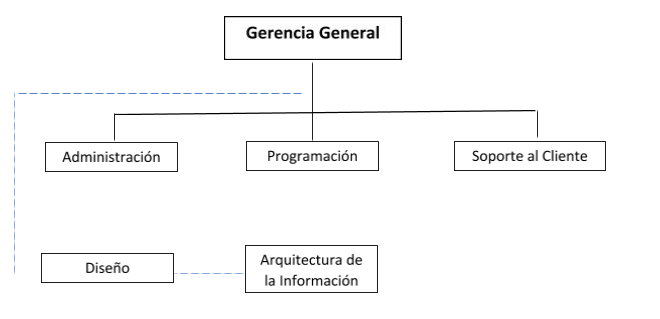
\includegraphics[scale=0.8]{organigrama}
\caption{Organigrama de la Empresa. Fuente: Elaboración propia.}
\label{fig:figura1}
\end{center}
\end{figure}

\chapter{Marco Teórico}
En el presente capítulo se definen las bases teóricas sobre las cuáles se apoya el proyecto. Para el desarrollo de la aplicación \textit{CPI} se utilizó Umbraco \cite{umbraco} como plataforma principal para de manejo de contenido (CMS) \cite{cmsBarker} y utilizando el patrón MVC \cite{mvcKrasner}.

\section{Bases Teóricas}

\subsection{CMS}
Un Sistema de Gestión de Contenido o CMS, por sus siglas en inglés \textit{Content Management System}, es un paquete de software que brinda cierto nivel de automatización de las tareas requeridas para administrar el contenido de manera efectiva. Un CMS permite a los usuarios crear nuevo contenido, editar contenido existente, y hacer el contenido accesible al público \cite{cmsBarker}.

Para los editores el CMS les permite crear contenido nuevo, editar contenido existente, realizar procesos en el contenido mediante una interfaz de edición (referida como \textit{back-end} que es la capa de acceso a los datos de la aplicación) y finalmente les permite colocar este contenido a disposición de otros usuarios en una interfaz (referida como el \textit{front-end}, es decir, la capa de presentación de la aplicación).

Un CMS permite el control del contenido, esto se refiere a que mantiene un constante seguimiento del contenido (donde se encuentra el contenido, quién puede acceder a él, y cómo se relaciona con otros contenidos). Por otro lado permite la reutilización del contenido (usar contenido en más de un lugar).

Una de las mayores ventajas de el uso de CMS es que facilita las tareas mencionadas anteriormente para usuarios que no tienen preparación técnica. En el caso de la aplicación \textit{CPI}, la mayoría de los usuarios no poseen conocimientos especializados en el área de computación, por lo cual es conveniente el desarrollo del sistema sobre un CMS

El CMS sobre el cual se trabajó para el desarrollo de la aplicación cuenta con funcionalidades que ya están implementadas que son necesarias para ésta, como la autenticación para los usuarios, permisología, interfaces que facilitan el manejo de la base de datos, entre otras cosas. Cuenta con gran variedad de paquetes, librerías y módulos que facilitan el desarrollo de la aplicación. 

\subsection{Modelo Cliente-Servidor}
Arquitectura de redes de computadoras ampliamente utilizado y que forma la base del uso de redes en gran medida, consta de dos entidades: un cliente y un servidor. El cliente le envía una solicitud al servidor y espera una respuesta. Luego, el servidor recibe la solicitud, lleva a cabo el trabajo requerido, o busca los datos solicitados y devuelve una respuesta al cliente \cite{redesTanenbaum}.

El servidor mantiene una relación de uno-a-muchos con los clientes, por otro lado ambos términos pueden ser vistos como “roles”, pues es posible que una máquina o proceso ejecute labores tanto de cliente como de servidor (por ejemplo, un servidor puede enviar una petición a otro servidor, si el mismo carece de los recursos que le fueron solicitados, convirtiéndose así en un cliente). Es importante destacar que los términos “cliente” y “servidor” pueden referirse tanto a máquinas como a programas o procesos. Esta arquitectura es ampliamente utilizada en aplicaciones web.

\subsection{MVC}
MVC, siglas para Modelo-Vista-Controlador, es un patrón de software utilizado ampliamente en la actualidad. Consiste en separar los datos de la aplicación (Modelo), la interfaz con el usuario (Vista), y la lógica de control (Controlador) en tres componentes distintos. Al realizar esta separación se reduce la complejidad del diseño arquitectónico y se incrementa la flexibilidad, la reusabilidad y mantenimiento del código. Adicionalmente, se pueden realizar cambios sobre un componente sin afectar a los demás, lo cual permite que cada componente tenga ciclos de desarrollo independientes del resto \cite{mvcKrasner}. 

Cabe destacar que este patrón es usado frecuentemente en el desarrollo de aplicaciones web, por lo que resulta bastante sencillo aplicarlo al modelo cliente-servidor utilizado en la aplicación. \textit{CPI} fue desarrollado usando una plataforma de desarrollo web basada en .NET que implementa este patrón.

\subsection{API}
Un API, llamado así por sus siglas en inglés para \textit{Application Programming Interface} (Interfaz de Programación de Aplicaciones), es un conjunto de comandos, funciones, protocolos y objetos que permiten exponer los datos de una aplicación de software, establecen las reglas y los mecanismos a través de los cuales se puede tener acceso a estos datos. También permite la interacción con algún software externo \cite{apiChristensson}.

El API sirve como intermediario entre dos aplicaciones, por ejemplo una aplicación dispone del API de otra para obtener los datos que se encuentran en la última y usarlos para proveer algún servicio a sus usuarios. En el caso de \textit{CPI} se desarrolló un API para poder acceder a datos de la aplicación.

\subsection{Servicio Web} \label{WebService}
Un servicio web es una aplicación o fuente de datos a la que se puede acceder a través de un protocolo web estándar, diseñado para soportar interacción máquina-máquina a través de una red, proveen una vía estándar para la comunicación entre distintas aplicaciones de software ejecutadas en distintas plataformas y ambientes. La mayoría de los servicios web proporcionan un API, para que se puedan acceder a los datos \cite{webServiceChristensson}.

Para la aplicación \textit{CPI} en el desarrollo se incluyó un módulo de servicios web, el cual permite el acceso a datos de la aplicación.

\subsection{REST}
Transferencia de Estado Representacional o REST, por sus siglas en inglés, es un estilo de arquitectura para sistemas de hipermedia distribuidos (como la \textit{World Wide Web} o red informática mundial) que define una serie de restricciones que, cuando se aplican en conjunto, enfatizan la escalabilidad de interacciones entre componentes, la generalidad de las interfaces y el despliegue independiente de componentes \cite{restFielding}.

Las restricciones definidas para los sistemas REST son las siguientes:

\begin{enumerate}
   \item \textbf{Separación Cliente-Servidor} el cliente y el servidor actúan independientemente, la interacción entre ellos ocurre solo a través de solicitudes que realiza el cliente, y las respuestas que envía el servidor como una reacción a una solicitud. El servidor solo envía información cuando ésta es solicitada por algún cliente.
   \item \textbf{Sin estado (\emph{stateless} en inglés)} el servidor no guarda información de ningún usuario que use los servicios del sistema. Cada solicitud individual contiene toda la información necesaria para ser ejecutada y enviar una respuesta, independientemente de todas las demás solicitudes que sean atendidas.
   \item \textbf{Permite el uso de memoria caché} la respuesta debe estar explícita o implícitamente etiquetada como \textit{cacheable} (se puede guardar en alguna memoria caché) o \textit{non-cacheable} (no se puede guardar en ninguna memoria caché). La ventaja del uso de memoria caché es que se pueden eliminar parcial o completamente algunas interacciones mejorando así el rendimiento del sistema.
   \item \textbf{Interfaz uniforme} cada solicitud al servidor debe tener los mismos componentes:
        \begin{itemize}
            \item Identificador del recurso deseado (en el caso de aplicaciones web este identificador puede ser el URL).
            \item Respuesta del servidor que debe incluir suficiente información para que el cliente pueda modificar el recurso (la información necesaria para que el servidor pueda llevar a cabo la solicitud y toda respuesta del servidor debe tener la información necesaria para que el cliente la entienda.
            \item Usar hipermedia como motor del estado de la aplicación, lo que quiere decir que el servidor debe poder informar al cliente las formas en las que puede cambiar el estado de la aplicación a través de enlaces de hipermedia, una página web específica se puede considerar un estado de la aplicación y enlaces incluidos en esa página se consideran transiciones a otros estados de la aplicación.
        \end{itemize}
    \item \textbf{Sistema por capas} entre el cliente que realiza una solicitud y el servidor que envía la respuesta final puede haber varios servidores, por ejemplo, puede haber un servidor que proporcione una capa de seguridad, otro una capa de memoria caché, y otros con otras funcionalidades. Estos servidores intermedios no deben afectar ni la solicitud ni la respuesta. Además, cada transacción (envío de la solicitud por el cliente y la subsiguiente respuesta) debe ser transparente para el cliente, es decir, el cliente no tiene conocimiento de las capas intermedias por las que pasan la solicitud y la respuesta.
\end{enumerate}

Se dice que un servicio web o el API de un servicio web es \textit{RESTful} cuando cumple con todas estas restricciones. El proyecto presente se desarrolló adhiriéndose a estas restricciones.

\subsection{SAAS}

Un Software como Servicio o SAAS, por sus siglas en inglés \textit{Software as a Service}, es un modelo para la distribución de software donde los clientes acceden al software a través de Internet. En SaaS, un proveedor de servicios aloja la aplicación en su centro de datos y un cliente accede a ella a través de un navegador web estándar \cite{saas}.
\chapter{Marco Tecnológico}
En el presente capítulo se muestran las herramientas necesarias para el desarrollo del proyecto, de tal manera que el lector pueda comprender los conceptos y tecnologías asociadas con la elaboración del mismo. 

\section{Lenguajes}
\subsection{C\#}
C\# es un lenguaje de programación desarrollado por Microsoft introducido en el año 2002, tiene seguridad de tipos y es orientado a objetos, el cual que permite a los desarrolladores crear una variedad de aplicaciones seguras y robustas que son ejecutadas en .NET Framework. Se puede usar C\# para crear aplicaciones cliente de Windows, servicios CML, componentes distribuidos, aplicaciones de bases de datos, aplicaciones cliente-servidor como es el caso de \textit{CPI} (la cual usa este lenguaje para desarrollar el código del \textit{back-end}) , entre otras \cite{cSharpMicrosoft}.

\subsection{HTML}
HTML por sus siglas en inglés \textit{Hypertext Markup Language} , es el lenguaje de marcado central de la \textit{World Wide Web} que es la red informática mundial. Originalmente, HTML fue diseñado principalmente para describir semánticamente documentos científicos. Sin embargo, la generalidad de su diseño ha permitido que se adapte, en la actualidad, para describir otros tipos de documentos e incluso aplicaciones \cite{htmlW3C}.

Todas las vistas de la aplicación \textit{CPI} fueron definidas por este lenguaje.


\subsection{CSS}
CSS por sus siglas en inglés \textit{Cascading Style Sheets} (Hojas de Estilo en Cascada), es el lenguaje para describir la presentación de páginas web (colores, diseños, fuentes, etc), permite a los usuarios agregar estilos a documentos estructurados como HTML. Al permitir la separacion del estilo de presentacion del contenido de los documentos, se facilita el mantenimiento de los sitios, el intercambio de hojas de estilo entre páginas y la personalización  de páginas en diferentes entornos \cite{cssW3C}.

\subsection{JavaScript}
JavaScript es un lenguaje de programación  interpretado comúnmente utilizado para el desarrollo web. Originalmente fue desarrollado por Netscape para crear contenido dinámico, control de multimedia, animación de imágenes, entre otras cosas a los sitios web.

Es un lenguaje de \textit{scripting} del lado del cliente, lo que significa que el código fuente es procesado por el navegador web del cliente y no en el servidor web \cite{javaScriptChristensson}.

\subsection{ASP.NET Razor}
Razor es un lenguaje de marcado, no es un lenguaje de programación, que permite incluir código basado en servidor (Visual Basic y C\#) en páginas web. 

El código basado en servidor puede crear contenido web dinámico sobre la marcha, mientras que una página web se escribe en el navegador. Cuando se hace un llamado a una página web, el servidor ejecuta el código basado en servidor dentro de la página antes de devolver la página al navegador, y al ejecutarse en el servidor, este código puede realizar tareas complejas.
 
Razor se basa en ASP.NET y está diseñado para crear aplicaciones web. Tiene el poder del marcado ASP.NET tradicional, pero es más fácil de usar y más fácil de aprender \cite{aspRazorW3school}.


\section{Frameworks}
\subsection{ASP.NET}
ASP.NET es un modelo de desarrollo Web unificado que incluye los servicios necesarios para crear aplicaciones Web de clase empresarial con un mínimo de codificación. ASP.NET es parte de .NET Framework y al codificar las aplicaciones en ASP.NET se tiene acceso a las clases de .NET Framework \cite{aspMicrosoft}.

\subsection{ASP.NET MVC}
ASP.NET MVC es un marco de trabajo para crear aplicaciones web escalables y basadas en estándares que usan patrones de diseño bien establecidos (patrón MVC) y el poder de ASP.NET y .NET Framework \cite{aspmvcMicrosoft}.

Para el desarrollo de uno de los módulos de la aplicación \textbf{CPI\_Core}, se utilizó este marco de trabajo, en donde se encuentran los controladores de la misma.

\subsection{ASP.NET Web Api}
ASP.NET Web API es un marco de trabajo que facilita la creación de servicios HTTP que llegan a una amplia gama de clientes, incluidos navegadores y dispositivos móviles. ASP.NET Web API es una plataforma ideal para crear aplicaciones RESTful en .NET Framework \cite{aspWebAPIMicrosoft}.

Para el desarrollo de uno de los módulos de la aplicación \textbf{CPI\_API}, se utilizó este marco de trabajo, en donde se implementaron los servicios del API para acceder a información del sistema (ver Sección \ref{WebService}) de la aplicación web.

\subsection{Umbraco}
Umbraco es un Sistema de Gestión de Contenido de código abierto gratuito desarrollado sobre ASP.NET, la primera versión de código abierto de Umbraco se lanzó el 16 de febrero del año 2005 \cite{umbraco}.

El principal objetivo de esta plataforma es brindar flexibilidad para que se puedan editar y hacer las cosas de la manera en la que se necesiten realizar, tiene todas las funcionalidades necesarias para desarrollar aplicaciones web como: la autenticación de usuarios, permisología, interfaces para manejar la base de datos, entre muchas más. Además para agregar funcionalidades extras a la versión básica de Umbraco cuenta con un repositorio de paquetes y extensiones que proveen variedad de librerías y módulos para facilitar el desarrollo del sistema. 

IKêls tiene varios años de experiencia desarrollando aplicaciones web usando Umbraco, por lo que resultó de mucha ayuda para el desarrollo de la aplicación. \textit{CPI} fue desarrollada sobre Umbraco v7.10.4


\section{Control de Versiones}
\subsection{Git}
Git es un sistema de control de versiones distribuido de código abierto y gratuito, diseñado para manejar desde proyectos pequeños hasta proyectos muy grandes con rapidez y eficiencia \cite{git}. Fue diseñado por Linus Torvalds en el año 2005 pensando en la eficiencia y la confiabilidad del mantenimiento de versiones de aplicaciones para facilitar el trabajo de varios desarrolladores sobre un mismo código fuente. Permite llevar el registro de los cambios de archivos y sincronizar el trabajo que varias personas realizan sobre archivos compartidos.

\section{Manejador de Base de Datos}
\subsection{SQL Server}
SQL Server es una parte central de la plataforma de datos de Microsoft. SQL Server es un líder de la industria en sistemas operativos de gestión de bases de datos (\textit{ODBMS})\cite{sqlServerMicrosoft}. Entre las tecnologías que tiene SQL Server la que se utilizó para la aplicación fue el motor de base de datos, el cual es el servicio principal para almacenar, procesar y proteger datos. El motor de base de datos proporciona acceso controlado y rápido procesamiento de transacciones para cumplir con los requisitos de las aplicaciones que requieren los datos más exigentes dentro de su empresa. 

\section{Entorno de Trabajo}
\subsection{Visual Studio}
Visual Studio es un entorno de desarrollo integrado que permite editar, depurar, compilar código para luego publicar una aplicación \cite{visualStudioMicrosoft}. Este entorno de desarrollo (\textit{IDE}) incluye una gran cantidad de funcionalidades para facilitar el desarrollo de software, entre las cuales están la depuración del código con información detallada de las variable y otras entidades del programa, instrucciones de compilación complejas para la aplicación, descarga y actualización paquetes y librerías, integración con Git, \textit{IntelliSense} de Microsoft como ayuda de codificación y la depuración de una aplicación para ver el valor de una variable durante la ejecución del programa y para la completación de código usando el contexto de la aplicación (clases, relaciones y métodos), entre otras.


\section{JSON}
JSON por sus siglas en inglés \textit{JavaScript Object Notation} es una sintaxis de texto que facilita el intercambio de datos estructurados entre todos los lenguajes de programación. Está basado en un subconjunto del lenguaje JavaScript. Utiliza en su sintaxis llaves, corchetes, dos puntos y comas lo cual es útil en muchos contextos y aplicaciones \cite{json}. Está constituido por dos estructuras:

\begin{itemize}
	\item Una colección de pares de nombre/valor. En varios lenguajes esto es conocido como un objeto, registro, estructura, diccionario, tabla hash, lista de claves o un arreglo asociativo.
    \item Una lista ordenada de valores. En la mayoría de los lenguajes, esto se implementa como arreglos, vectores, listas o secuencias.
\end{itemize}

\section{Ajax}
Ajax por sus siglas en inglés \textit{Asynchronous JavaScript And XML} es una combinación de tecnologías de desarrollo web utilizadas para crear sitios web dinámicos. Los sitios que utilizan Ajax combinan JavaScript y XML para mostrar contenido dinámico \cite{ajaxChristensson}. Con “asíncrono” se refiere a la forma en la que se realizan las solicitudes al servidor web, ya que al enviar una solicitud al servidor web, éste puede recibir datos que luego pueden ser mostrados en la página web.

\section{Highcharts}
Highcharts es una biblioteca de gráficos escrita en JavaScript puro, que ofrece una manera fácil de agregar gráficos interactivos a su sitio web o aplicación web. Fue lanzado en el año 2009, \cite{highcharts}. 

En la aplicación \textit{CPI} se usó para realizar los gráficos de barra, boxplot y dispersión que muestran los reportes de precios de los productos, de los productos por categorías, y el histórico de precios de un producto.


\section{DataTables}
DataTables es un complemento para la biblioteca jQuery de Javascript. Es una herramienta altamente flexible, y su objetivo es mejorar la accesibilidad de los datos en las tablas HTML \cite{dataTables}. 

Este complemento fue usado para cada una de las tablas de la aplicación \textit{CPI}.



\chapter{Marco Metodológico}
En este capítulo se explicará la metodología que se utilizó para el desarrollo del proyecto, que fue necesaria usar para cumplir con los objetivos planteados, conocida como Scrum. A continuación se describirá el marco de desarrollo, las actividades y resultados de cada una de las etapas de esta metodología.

\section{¿Qué es Scrum?}
Scrum es un marco de trabajo para desarrollar, entregar y mantener productos complejos, en el cual las personas pueden abordar problemas complejos adaptativos, y a su vez entregar productos del máximo valor posible productiva y creativamente. Empezó a ser usado desde principios de los años 90. Scrum es un marco de trabajo dentro del cual se pueden emplear varios procesos y técnicas. El marco de trabajo Scrum consiste en los Equipos Scrum y sus roles, eventos, artefactos y reglas asociadas \cite{scrumSchwaber}.

Usando correctamente este marco de trabajo se puede mostrar la eficacia relativa de las técnicas de la gestión del producto y las técnicas de trabajo, de manera que a medida que va pasando el tiempo se pueda mejorar el producto, el equipo y el entorno de trabajo. Para que esto suceda es necesario que cada componente que interactúa dentro de Scrum cumpla con su propósito específico.

\section{Usos de Scrum}
Scrum inicialmente fue desarrollado para la gestión y desarrollo de productos. Se ha usado principalmente para:

\begin{enumerate}
	\item Investigar e identificar mercados viables, tecnologías y capacidades de productos.
	\item Desarrollar productos y mejoras.
	\item Liberar productos y mejoras tantas veces como sea posible durante el día.
	\item Desarrollar y mantener ambientes en la Nube (en línea, seguros, bajo demanda) y otros entornos operacionales para el uso de productos.
	\item Mantener y renovar productos.
\end{enumerate}

\section{Equipo de Scrum}

El equipo Scrum está conformado por el Dueño del Producto (\textit{Product Owner}), el Equipo de desarrollo (\textit{Development Team}) y un \textit{Scrum Master}. Los equipos Scrum son autoorganizados y multifuncionales. Los equipos autoorganizados eligen la mejor forma de llevar a cabo su trabajo y no son dirigidos por personas externas al equipo. Los equipos multifuncionales tienen todas las competencias necesarias para llevar a cabo el trabajo sin depender de otras personas que no son parte del equipo. El modelo de equipo en Scrum está diseñado para optimizar la flexibilidad, la creatividad y la productividad \cite{scrumSchwaber}.

\subsection{Dueño del Producto} \label{productOwner}
Es el responsable de maximizar el valor del producto resultante del trabajo del Equipo de Desarrollo. Es la única persona responsable de gestionar la Lista del Producto (\textit{Product Backlog}), esto incluye:
\begin{itemize}
\item Expresar claramente los elementos de la lista.
\item Ordenar los elementos de la lista, para alcanzar objetivos y misiones de manera eficiente.
	\item Optimizar el valor del trabajo que el Equipo de Desarrollo realiza.
	\item Asegurar que la lista sea visible, transparente y clara para todos y que muestra aquello en lo que el equipo trabajará a continuación.
	\item Asegurar que el Equipo de Desarrollo entiende los elementos de la Lista del Producto al nivel necesario.
\end{itemize}

\begin{itemize}
    \item Expresar los items del \emph{Product Backlog}
\end{itemize}

\subsection{Equipo de Desarrollo}
El Equipo de Desarrollo está conformado por profesionales que realizan el trabajo de entregar un Incremento (ver Sección \ref{incremento}) de producto “Terminado” que potencialmente se puede poner en producción al final de cada Sprint (ver Sección \ref{sprint}). Cabe destacar que solo los miembros del Equipo de Desarrollo participan en la creación del Incremento, ellos se organizan y gestionan su propio trabajo. Los Equipos de Desarrollo tienen las siguientes características: 

\begin{itemize}
	\item Son autoorganizados. Nadie (ni siquiera el Scrum Master) indica al Equipo de Desarrollo cómo convertir elementos de la Lista del Producto en Incrementos de funcionalidad potencialmente desplegables.
	\item Los Equipos de Desarrollo son multifuncionales, esto es, como equipo cuentan con todas las habilidades necesarias para crear un Incremento de producto.
	\item Scrum no reconoce títulos para los miembros de un Equipo de Desarrollo independientemente del trabajo que realice cada persona
	\item Los Miembros individuales del Equipo de Desarrollo pueden tener habilidades especializadas y áreas en las que estén más enfocados, pero la responsabilidad recae en el Equipo de Desarrollo como un todo. 
\end{itemize}


\subsection{Scrum Master} \label{scrumMaster}

El Facilitador (o \emph{Scrum Master}) es el responsable de promover y apoyar Scrum como está definido en la Guía de Scrum \cite{scrumSchwaber}. Esto lo logran ayudando a todo el Equipo Scrum a entender la teoría, práctica, reglas y valores de Scrum \cite{scrumSchwaber}.

\section{Eventos de Scrum}

Para minimizar y regularizar la necesidad de reuniones no definidas en Scrum existen eventos predefinidos. Los eventos son bloques de tiempo (\textit{label-boxes}), de tal modo que todos tienen una duración máxima. En el caso de un Sprint (ver Sección \ref{sprint}), su duración es fija y no puede acortarse ni alargarse, el resto de eventos pueden terminar antes siempre y cuando se cumplan con el objetivo del evento \cite{scrumSchwaber}.


\subsection{Sprint} \label{sprint}
El Sprint es el corazón de Scrum, es un bloque de tiempo de aproximadamente un mes de duración durante el cual se crea un Incremento (ver Sección \ref{incremento}) del producto “Terminado” utilizable y potencialmente desplegable. Cada nuevo Sprint comienza inmediatamente después de la finalización del Sprint anterior \cite{scrumSchwaber}.

Los Sprint están compuestos por la Planificación del Sprint (\textit{Sprint Planning}), los Scrums Diarios (\textit{Daily Scrums}), el trabajo de desarrollo, la Revisión del Sprint (\textit{Sprint Review}), y la Retrospectiva del Sprint (\textit{Sprint Retrospective}). 

\section{Artefactos de Scrum}
Los artefactos de Scrum representan trabajo o valor en diversas formas que son útiles para proporcionar transparencia y oportunidades para la inspección y adaptación. Los artefactos definidos por Scrum están diseñados específicamente para maximizar la transparencia de la información clave, necesaria para asegurar que todos tengan el mismo entendimiento del artefacto \cite{scrumSchwaber}.

\subsection{Lista de Producto} \label{productBacklog}
La Lista de Producto es una lista ordenada de los objetivos y requisitos que son necesario en el producto. El Dueño de Producto (Product Owner) es el responsable de esta lista, incluyendo su contenido, disponibilidad y ordenación. La Lista de Producto va cambiando constantemente a medida de que el producto y el entorno en el que se usará también lo hacen, es decir cambia mientras se van identificando necesidades para que el producto pueda ser adecuado, competitivo y útil. La Lista de Producto enumera todas las características, funcionalidades, requisitos, mejoras y correcciones que constituyen cambios a realizarse sobre el producto para entregas futuras \cite{scrumSchwaber}.

\subsection{Lista de Pendientes del Sprint} \label{sprintBacklog}
La lista de Pendientes del Sprint es el conjunto de elementos seleccionados para realizar en el Sprint de la Lista de Productos, más un plan para entregar el Incremento (ver Sección \ref{incremento} del producto y cumplir los objetivos del Sprint \cite{scrumSchwaber}. Esta lista la realiza el Equipo de Desarrollo y se basa en la funcionalidad que formará parte del próximo Incremento.

\subsection{Incremento} \label{incremento}

El Incremento es la suma de todos los elementos de la Lista de Producto completados durante un Sprint y el valor de los incrementos de todos los Sprints anteriores. Al final de un Sprint el nuevo Incremento debe estar “Terminado”, lo cual significa que está en condiciones de ser utilizado y que cumple la Definición de “Terminado” del Equipo Scrum (cada equipo tiene su propia definición de un producto o Incremento terminado). El incremento es un paso hacia una visión o meta. El incremento debe estar en condiciones de utilizarse sin importar si el Dueño de Producto decide liberarlo o no \cite{scrumSchwaber}.



\chapter{Desarrollo} \label{development}
En este capítulo se presentan las actividades realizadas durante el desarrollo del proyecto correspondientes al período de pasantías Abril-Septiembre 2018. El proyecto inicialmente tenía planteado el desarrollo de cuatro módulos:
\begin{enumerate}
	\item Módulo de administración de cadenas, tiendas, zonas, productos y categorías: En principio el desarrollo de este módulo consistía en el desarrollo de la interfaz gráfica para cada una de estas entidades para la creación, edición y eliminación de registros, sin embargo faltaron las entidades tiendas y zonas, la asignación de tiendas a cadenas, el cual no se realizó, asignar productos a categorías y finalmente crear el listado de los registros de productos con mecanismo de búsqueda.
	\item Módulo de administración de precios: Este módulo incluye la interfaz de creación, edición y eliminación de registros, el desarrollo de un mecanismo para importar los precios en lote usando un archivo en formato Microsoft Excel y de igual manera importar por lote mediante webservice desde una fuente externa en formato JSON, sin embargo ésta última no se realizó.
	\item Módulo de generación de reportes: Para este módulo se planteó el desarrollo de la funcionalidad de generar reportes comparativos para: 
    \begin{itemize}
        \item Gráfico de dispersión de precios / categorías.
        \item Gráfico de barras para un producto seleccionado separando precio normal y oferta.
        \item Gráfico tipo box-plot para el histórico de precios de un producto.
	\end{itemize}
	Implementar un mecanismo automático para generar reportes de manera frecuente y enviar alertas de correo con el resultado, y finalmente un mecanismo para exportar los reportes en un formato tipo tabla en Microsoft Excel, sin embargo estas dos últimas funcionalidades se decidieron dejar para una próxima versión del sistema, ya que el desarrollo de la primera funcionalidad tomó más tiempo del pensado, debido a su complejidad.
	\item Módulo de preferencias para usuario: Este módulo no se desarrolló, debido a que el mismo tenía directa relación con las dos últimas funcionalidades del módulo anterior y al no desarrollarlas, este módulo no tenía sentido. 
\end{enumerate}
    El proyecto se dividió en 3 Fases :
\begin{itemize}
   \item Fase de Inducción, en la cual se hace la introducción del proyecto, el pasante se familiariza con las herramientas y tecnologías necesarias para realizar el proyecto.
   \item Fase de Desarrollo la cual se divide en 5 Sprints, en esta fase se hace la implementación de los diferentes módulos de la aplicación.
   \item Fase de Documentación en la cual se realiza parte de la documentación necesaria para la aplicación.
\end{itemize}
A continuación, se explicará en detalle en qué consiste cada Fase.

\section{Inducción}
Durante esta Fase el pasante realizó un proceso de familiarización con la empresa junto con el estudio de herramientas y lenguajes de trabajo que fueron empleados a lo largo del desarrollo del proyecto.
Realizó varios cursos tutoriales (Umbraco Course level 1, Learn ASP.NET MVC de Microsoft Virtual Academy, entre otros),  y utilizó recursos (guía de Umbraco) que la empresa proporcionó para tener los conocimientos necesarios para llevar a cabo el proyecto. Además investigó sobre herramientas como: ASP.NET, SQL Server, Highcharts y Visual Studio.

La duración de esta fase fue de una semana, sin embargo, el pasante tuvo que mantenerse en constante búsqueda de recursos e investigar sobre la marcha sobre herramientas o conceptos nuevos, los cuales se fueron necesitando en el camino. Todo este proceso fue sumamente útil y de gran aprendizaje ya que la mayoría de las herramientas utilizadas para el desarrollo del proyecto eran nuevas y muchos de los conceptos se investigaron a profundidad.

\section{Desarrollo}
La Fase de desarrollo de la aplicación se realizó en cinco Sprints, los cuales tuvieron una duración en total de 17 semanas continuas. A continuación una descripción del trabajo realizado en cada uno.

\subsection{Primer Sprint}
Durante este Sprint se hizo el análisis y definición de los requerimientos de la aplicación, los cuales eran primero definir el alcance inicial de la aplicación (ver bla bla), definir la arquitectura a utilizar y por último la estructura de la base de datos. El pasante inició la familiarización de la versión actual de CPI junto con el dueño del producto para resolver las posibles dudas de la funcionalidad, o conceptos necesarios para entender la aplicación. Además se creó el repositorio de Git, el proyecto de Visual Studio y el sitio de Umbraco, y por último el Dueño del producto sugirió dos posibles plantillas de HTML que podrían ser utilizadas para las vistas de la aplicación y el pasante eligió la que era más adecuada visual y funcionalmente para la misma. 
\\
\\
\textbf{Actividades realizadas:}
\begin{itemize}
   \item Familiarización con la versión original de CPI. Esta actividad consistió principalmente en reuniones con el dueño del producto para aclarar dudas con respecto a los conceptos necesarios para entender la aplicación y sus funcionalidades.
   \item Elegir la arquitectura de la aplicación. El pasante junto con el Dueño del Producto decidieron utilizar el modelo de 4+1 Vistas de Philippe Kruchten.
   \item Definir los actores del sistema. En principio se definieron dos actores principales para la aplicación, \textit{Admin} (el administrador del sistema) y \textit{Retailer} (representantes de cadenas).
   \item Realizar una matriz de permisología de las funcionalidades de la aplicación. Lo que el pasante realizó fue listar todas las posibles funciones de cada uno de los módulos de aplicación y definir cuáles eran los permisos que tendrán cada uno de los actores.
   \item Elegir las entidades de la aplicación. El pasante basándose en la primera versión de la aplicación y junto el dueño del producto tomaron la decisión de cuáles serían las entidades que se manejarían desde la base de datos de Umbraco (cadenas) y cuáles en la base de datos de SQL Server (tiendas, zonas, productos, precios y categorías).
   \item Rediseñar la base de datos. Luego de decidir cuáles eran las entidades a trabajar en la base de datos de SQL Server el pasante junto con el Dueño del Producto decidieron cuál podría ser la nueva estructura de la base de datos. A continuación se muestra el Diagrama de la versión original de CPI (ver Figura \ref{fig:er_viejo}) y el Diagrama ER de la versión 2 de CPI (ver Figura \ref{fig:er_nuevo})
        \begin{figure}[hbt]
        \begin{center}
        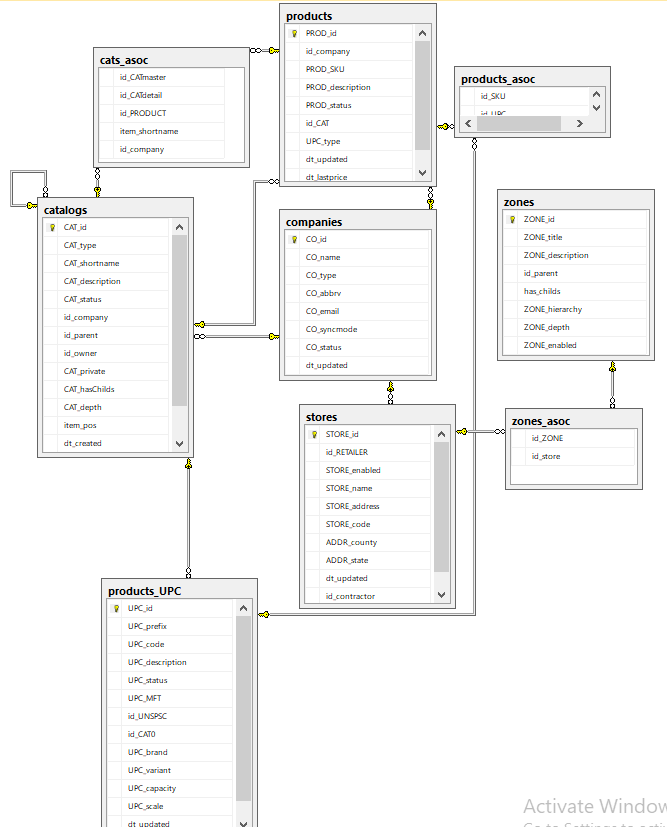
\includegraphics[scale=0.8]{er_viejo.png}
        \caption{Diegrama ER de la base de datos de la versión 1 de CPI.}
        \label{fig:er_viejo}
        \end{center}
        \end{figure}

        \begin{figure}[hbt]
        \begin{center}
        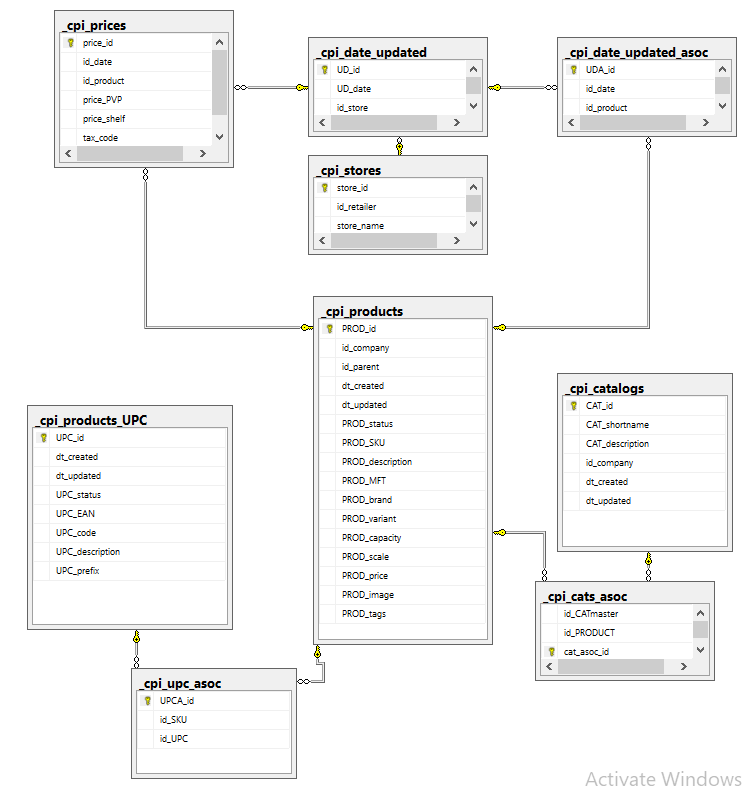
\includegraphics[scale=0.8]{er.png}
        \caption{Diagrama de la base de datos de la nueva versión de CPI.}
        \label{fig:er_nuevo}
        \end{center}
        \end{figure}
        \item Crear el proyecto en Visual Studio. 
        \item Crear el repositorio de Git. Para el proyecto se creó un repositorio llamado CPI el cual se utilizó para el control de versiones del proyecto. Para utilizar correctamente el repositorio el pasante tuvo que refrescar los comandos.
        \item Crear el sitio de Umbraco.
        \item Elegir la plantilla a utilizar para las vistas de la aplicación. El pasante junto con el Dueño del Producto eligieron entre dos posibles plantillas, la elegida fue la que más se acopló a las necesidades de la aplicación.
        \item Investigar sobre Datatables ya que fue el pluggin (complemento) elegido por el Dueño del Producto para manejar dinámicamente las tablas.
        \item Listar las vistas que tendrá la aplicación, según los módulos que se eligieron como alcance inicial.
    \end{itemize}
\textbf{Duración:} 2 semanas.

\subsection{Módulo de Administración de cadenas, productos y categorías (2da Iteración)}
Durante esta iteración se implementó la funcionalidad para el manejo de las principales entidades de la aplicación: cadenas, productos y categorías. En la cual se desarrolló una interfaz gráfica en el back end de Umbraco usando un paquete llamado Fluidity para el manejo de estas entidades en la base de datos. Se definieron los Doctypes y Datatypes para crear el contenido en Umbraco. Se inició el desarrollo de las vistas de la aplicación.

Al finalizar esta iteración fue posible manejar las entidades de la aplicación por medio del árbol de contenido de Umbraco o por medio de la interfaz gráfica de Fluidity. 

\textbf{Actividades realizadas:}
\begin{itemize}
   \item Definir los Doctypes para las entidades principales.
   \item Definir los Datatypes para las entidades principales.
   \item Desarrollar la interfaz de Fluidity para creación, edición y eliminación de registros de las entidades que se guardan en la base de datos de SQL Server.
   \item Iniciar desarrollo de las vistas de la aplicación.
   \item Realizar vista de listado de productos.
\end{itemize}


\textbf{Duración:} 3 semanas.

\subsection{Módulo de Generación de Reportes (3ra Iteración)}
En esta iteración se desarrolló parte de la funcionalidad de generación de reportes comparativos. Se realizó la vista de cada uno de los gráficos (barras y boxplot) que permiten la comparación de precios entre productos de una cadena, o productos que tienen en común distintas cadenas y además tablas que muestran información necesaria para cada uno de estos gráficos. Esta iteración tuvo una duración más larga de la planificada ya que para realizar cada uno de los gráficos se necesitaba traer datos de la base de datos y la traducción del código de la versión antigua a la nueva versión tomó más tiempo de lo esperado ya que no se encontraba bien documentada.


\textbf{Actividades realizadas:}
\begin{itemize}
   \item Desarrollar vista de gráfico de barras para un producto seleccionado de la lista de productos de la cadena, separando precio normal y oferta.
   \item Desarrollar vista de gráfico tipo boxplot para el precio histórico de un producto.
   \item Traducir scripts para traer datos de la base de datos.
   \item Mejorar código y funcionalidad que se desarrollaron en iteraciones anteriores.
\end{itemize}


\textbf{Duración:} 4 semanas.

\subsection{Continuación con el Módulo de Generación de Reportes (4ta Iteración)}
En esta Iteración se siguió el desarrollo de la generación de reportes completando el reporte de precios por categorías (gráfico de dispersión) y se mejoraron algunos aspectos de las otras iteraciones.

\textbf{Actividades realizadas:}
\begin{itemize}
   \item Desarrollar la vista del reporte de precios por categorías.
   \item Mejorar código de la aplicación.
\end{itemize}

\textbf{Duración:} 3 semanas.


\subsection{Refactorización (5ta Iteración)}
Al iniciar esta iteración se llegó a la conclusión que el desarrollo de la funcionalidad que se tenía hasta el momento no estaba siguiendo la estructura que realmente se quería tener en la solución de Visual Studio, ya que los controladores no estaban organizados correctamente según el patrón MVC. Además habian funciones que debían estar implementadas en \verb|CPI_API| pero se encontraba en \verb|CPI_Core| y se estaba utilizando el tipo de controlador incorrecto. Este inconveniente ocurrió por la falta de comunicación entre el dueño del producto y el desarrollador (pasante), sin embargo se hicieron las correcciones necesarias para corregir este imprevisto, sin embargo tomó tiempo extra que no se tenía planificado y por esta razón no se alcanzó a realizar parte de algunos módulos que ya se encontraban en la planificación.


\textbf{Actividades realizadas:}
\begin{itemize}
   \item Reorganizar los controladores de la aplicación.
   \item Refactorizar código en gran parte de la funcionalidad.
   \item Mejorar calidad del código.
\end{itemize}

\textbf{Duración:} 2 semanas.


\subsection{Módulo de Administración de precios (6ta Iteración)}
Esta fue la última Iteración de desarrollo, en la cual se implementó el módulo de administración de precios de productos. Se creó la interfaz gráfica usando Fluidity y además la funcionalidad para importar un lote de precios usando un archivo en formato MS Excel (CSV). Además se hicieron mejoras de código implementado en las iteraciones anteriores y correcciones de bugs.

\textbf{Actividades realizadas:}
\begin{itemize}
   \item Implementar la autenticación, inicio y cierre de sesión para el front end de la aplicación.
   \item Desarrollar interfaz gráfica para creación, edición y eliminación de registros.
   \item Mejorar código y corregir bugs.
\end{itemize}

\textbf{Duración:} 3 semanas.


\section{Documentación} \label{documentation}
Esta última fase del proyecto duró las últimas dos semanas del período de pasantía. Se realizó la documentación necesaria para la aplicación, se dejó expresado el estado final del sistema, se elaboraron los documentos de instalación de CPI y el Documento de Arquitectura de Software donde se detallan los componentes y casos de uso desarrollados de la aplicación.

\chapter*{Conclusiones y Recomendaciones}
\par Conclusiones aquí.
\nocite{*}
\bibliography{referencias}
%\appendix

\end{document}
